\documentclass{llncs}
\usepackage{amssymb}
\usepackage[utf8]{inputenc}
\usepackage{url}
\usepackage{graphicx}
\usepackage{caption}
\usepackage{subcaption}
\usepackage{epstopdf}
\usepackage{subfig}
\usepackage{float}
\usepackage{amsmath}
\usepackage{wrapfig}
\usepackage{fancyhdr} %Usado para configurar encabezado y pie de página
\usepackage{enumitem}
%\usepackage[tight,scriptsize,centerlast]{subfigure}
\usepackage{subfloat} 
%\usepackage{subfigure}



\pagestyle{empty}
\pagestyle{fancy}
%\rfoot{\thepage}

\begin{document}

\title{Pumas@Home 2019 Team Description Paper
\thanks{Acknowledgment: This work was supported by PAPIIT-DGAPA UNAM under Grant IG100915}}
\author{
	Jesus Savage 
	\and Reynaldo Martell 
	\and Hugo Estrada 
	\and Julio Cruz 
	\and Marco Negrete 
	%\and Jesus Cruz
	%\and Jose Cruz
	%\and Edgar Vazquez
	\and Jaime Marquez
	%\and Edgar Silva
	\and Manuel Pano 
	%\and Luis Alvarez
	%\and Mauricio Matamoros
	\and Julio Martinez
}
\institute{Bio-Robotics Laboratory, School of Engineering \\ National Autonomous University of Mexico \\
\texttt{http://biorobotics.fi-p.unam.mx}}
\maketitle


%%%%%%%%%%%%%
%%%  ABSTRACT  %%%
%%%%%%%%%%%%%
\begin{abstract}

This paper describes the service robot Justina of team Pumas that has participated in the @Home category of the RoboCup and RoCKIn, both of them international competitions; as well as our latest applied research. These competitions had influenced our architecture in the development of better systems for our service robots by developing algorithms to natural language understanding and the flat-and-textureless object manipulation.
In our robotics architecture, the VIrtual and Real roBOt sysTem (VIRBOT), the operation of service robots is divided into several subsystems, each of them has a specific functionality  that contributes to the final operation of the robot.
By combining symbolic AI with digital signal processing techniques a good performance of a service robot is obtained.

\end{abstract}

%%%%%%%%%%%%%%%
%%% INTRODUCTION %%%
%%%%%%%%%%%%%%%

\section{Introduction}

Service robots are hardware and software systems that assist humans to perform daily tasks in complex environments, to achieve this: they have to be able to understand spoken or gesture commands from humans; to be able to avoid static and dynamic obstacles while navigating in known and unknown environments; to be able to recognize and to manipulate objects and performing several other tasks that a person might request. 

Our team has been participated in the category @Home continuously since the start of this competition at the RoboCup in Bremen in 2006. Our team obtained the  fourth place and got the award for the best in Speech Recognition and Natural Language Understanding in Nagoya in 2017, last year, in the RoboCup 2018, the team obtained the second place.

The paper is organized as follows:
section \ref{sec:background} enumerates the hardware and software components of our robot
Justina; section \ref{sec:CurrentResearch}  presents overview of the latest research developments in our
laboratory; and finally, in section \ref{sec:conclusions}, the conclusions and future work are given.


\section{Justina's Robotics Architecture}\label{sec:background}
\subsection{Hardware Configuration}

Our service robot Justina, see figure \ref{fig:justina}, has the following components:\\

\begin{wrapfigure}{r}{0.5\textwidth}
	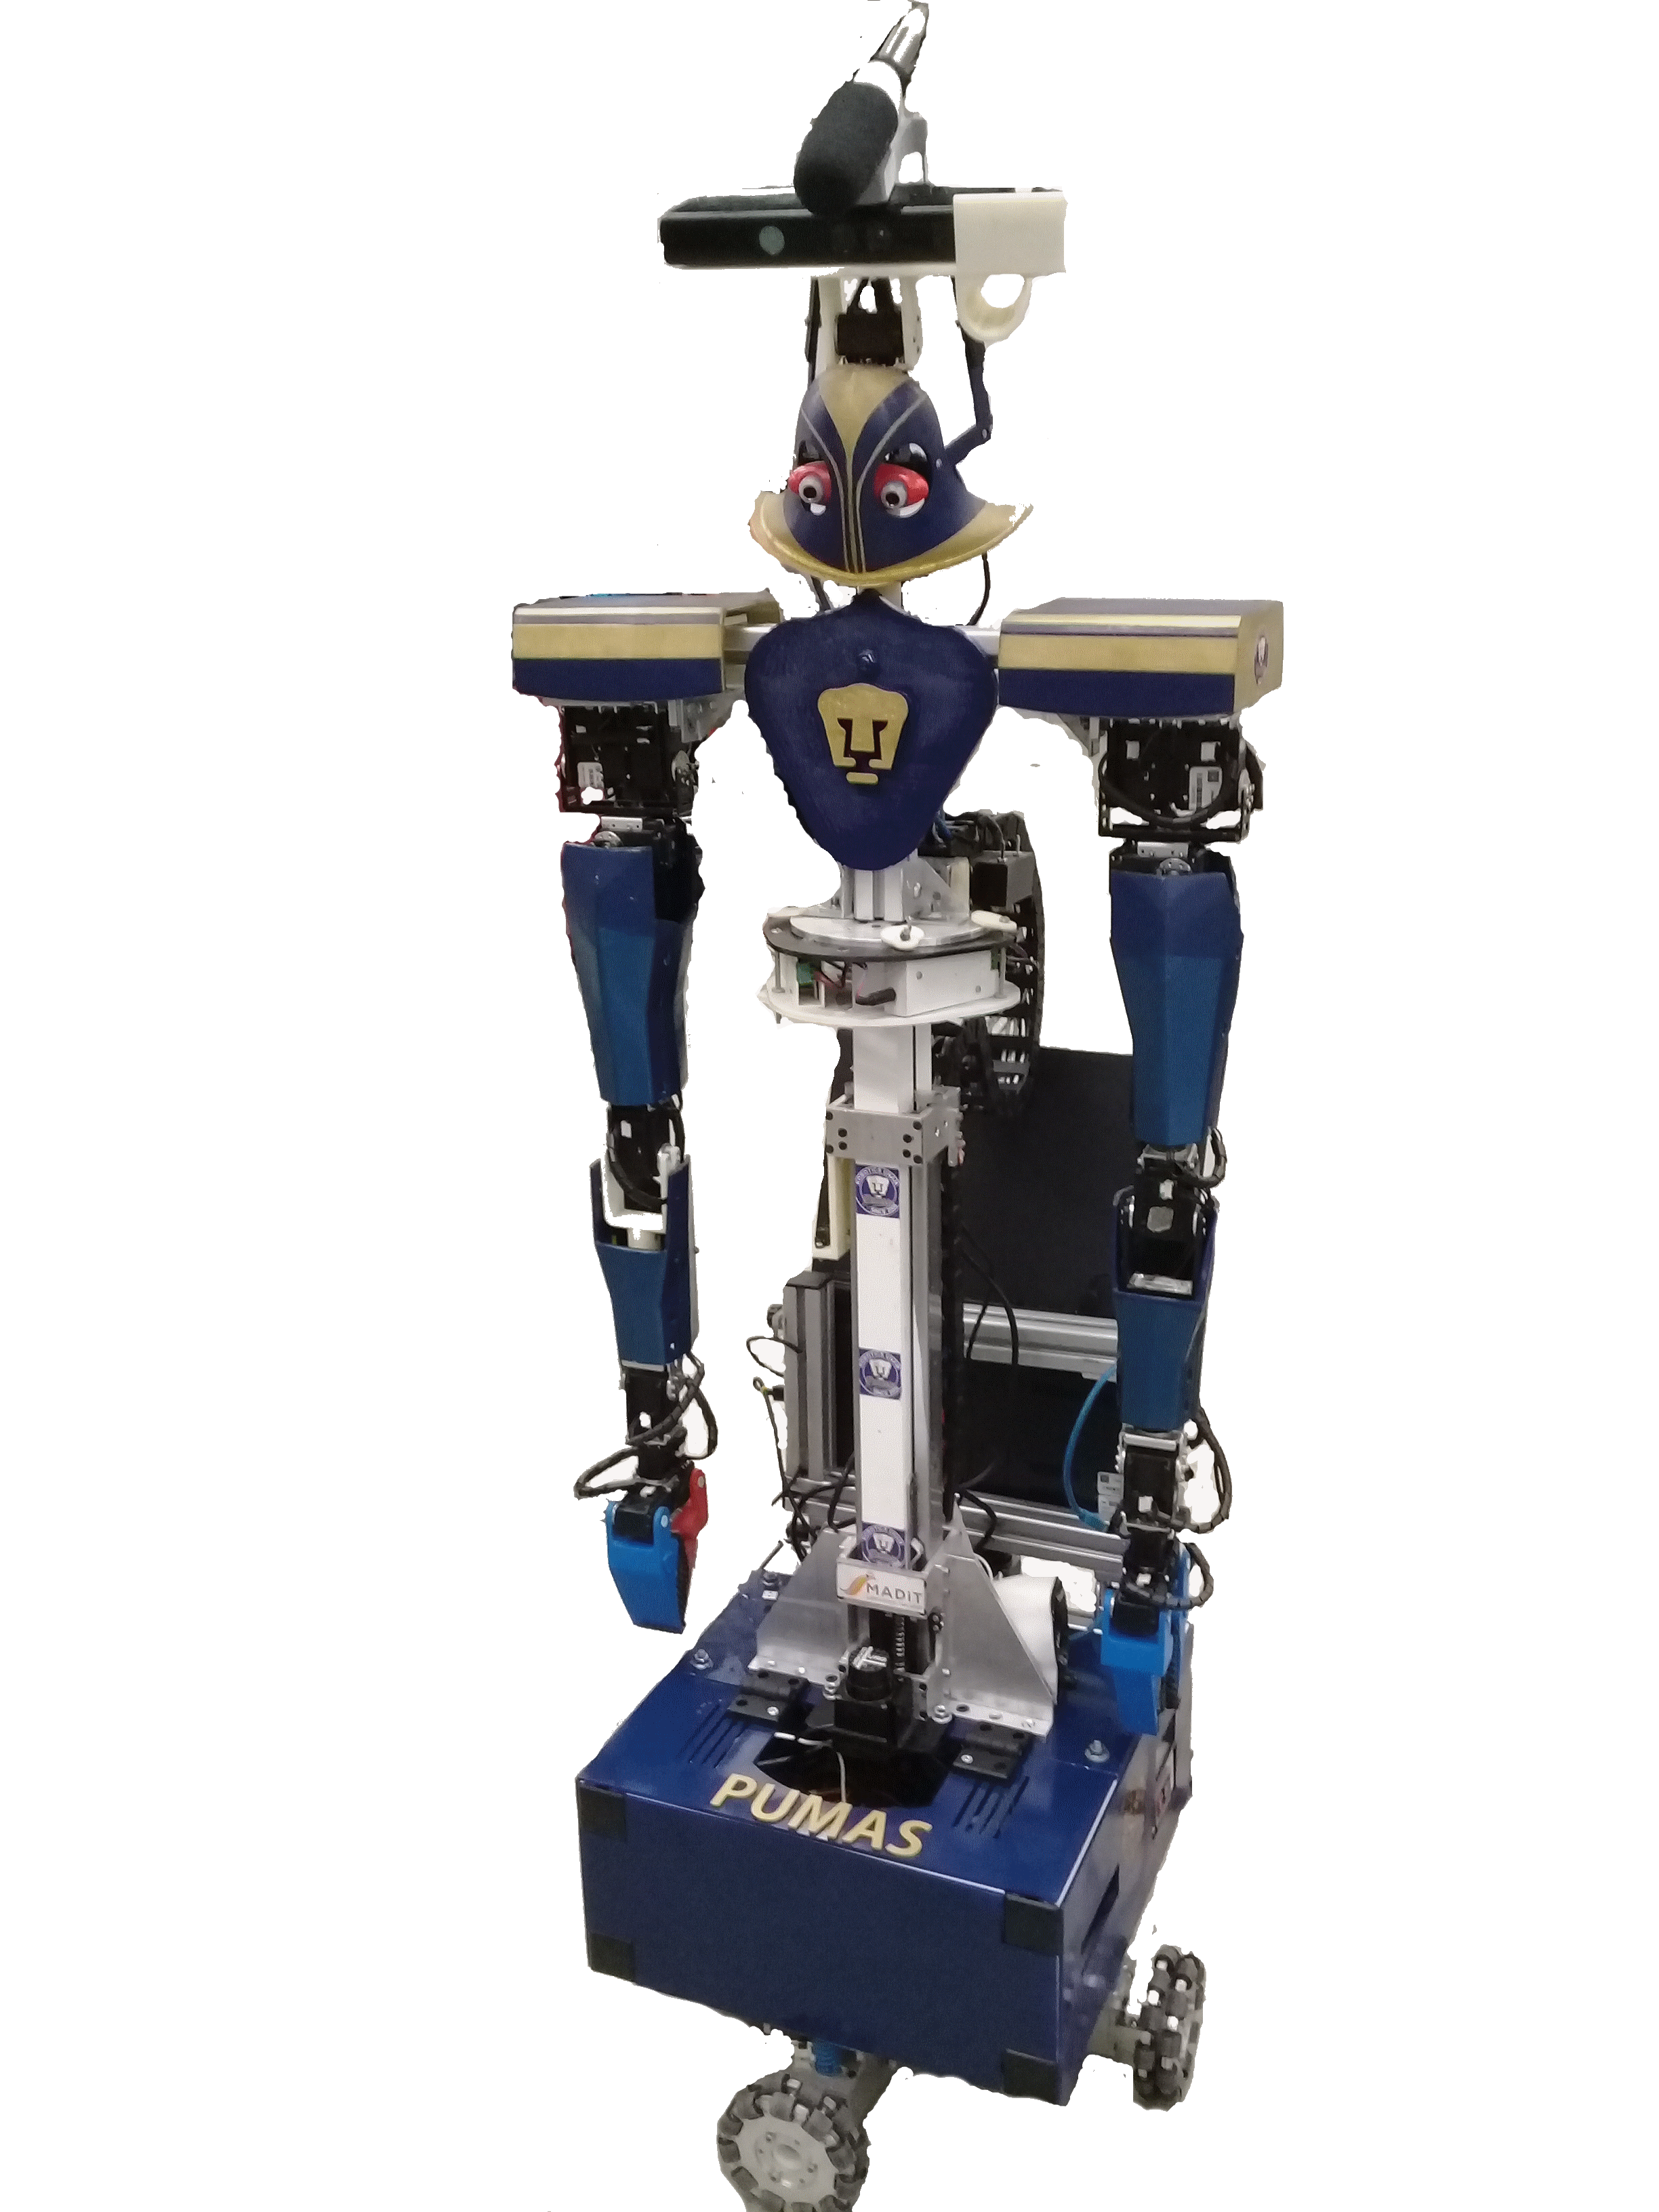
\includegraphics[angle=0, height=10cm, width=6cm]{Figures/ImagenNuevaJustina.png}
  \caption{Robot Justina}
  \label{fig:justina}
\end{wrapfigure}



HARDWARE:

\begin{itemize}
	\item \textbf{Mobile base:} Omnidirectional through differential pair configuration and omnidirectional wheels. 
	\item \textbf{Manipulators:} 2 x 7-DOF anthropomorphic arms with 10 Dynamixel servomotors each.
	\item \textbf{Head:} 2-DOF (Pan and tilt) built with Dynamixel servomotors.
	\item \textbf{Torso:} 1-DOF (Elevation) through a worm screw and a configuration of gears. 
	\item \textbf{Speakers:} Two speakers to generate synthetic speech.
	\item \textbf{RGB-D Camera:} Microsoft's Kinect sensor. 
	\item \textbf{RGB Camera:} Logitech Pro C920 Full HD.
	\item \textbf{Microphone:} Rode NTG2 directional microphone.
	\item \textbf{Array of Microphones:} An array of four microphones to detect sound sources.
	\item \textbf{Laser:} Hokuyo rangefinder URG-04LX-UG0.
	\item \textbf{Embbeded System:} NVIDIA Jetson TX2 to image processing.
\end{itemize}



\subsection{Software Configuration}
Our software configuration is based on the VIRBOT architecture \cite{virbot}, 
which provides a platform for the design and development of software for general purpose service robots, see figure \ref{fig:virbot}. 
The VIRBOT architecture is implemented in our robots through several modules that perform well defined tasks \cite{muller}, with a 
high level of interaction between them. The principal framework used for interaction is ROS, where a module is represented by one or 
several ROS's nodes. Also, for modules using the Microsoft operating system, we use our own middleware called Blackboard to
link them with ROS nodes running on Linux.
In the following sections are explained each of the layers of the VIRBOT system.


\begin{figure}[h]
	\centering
	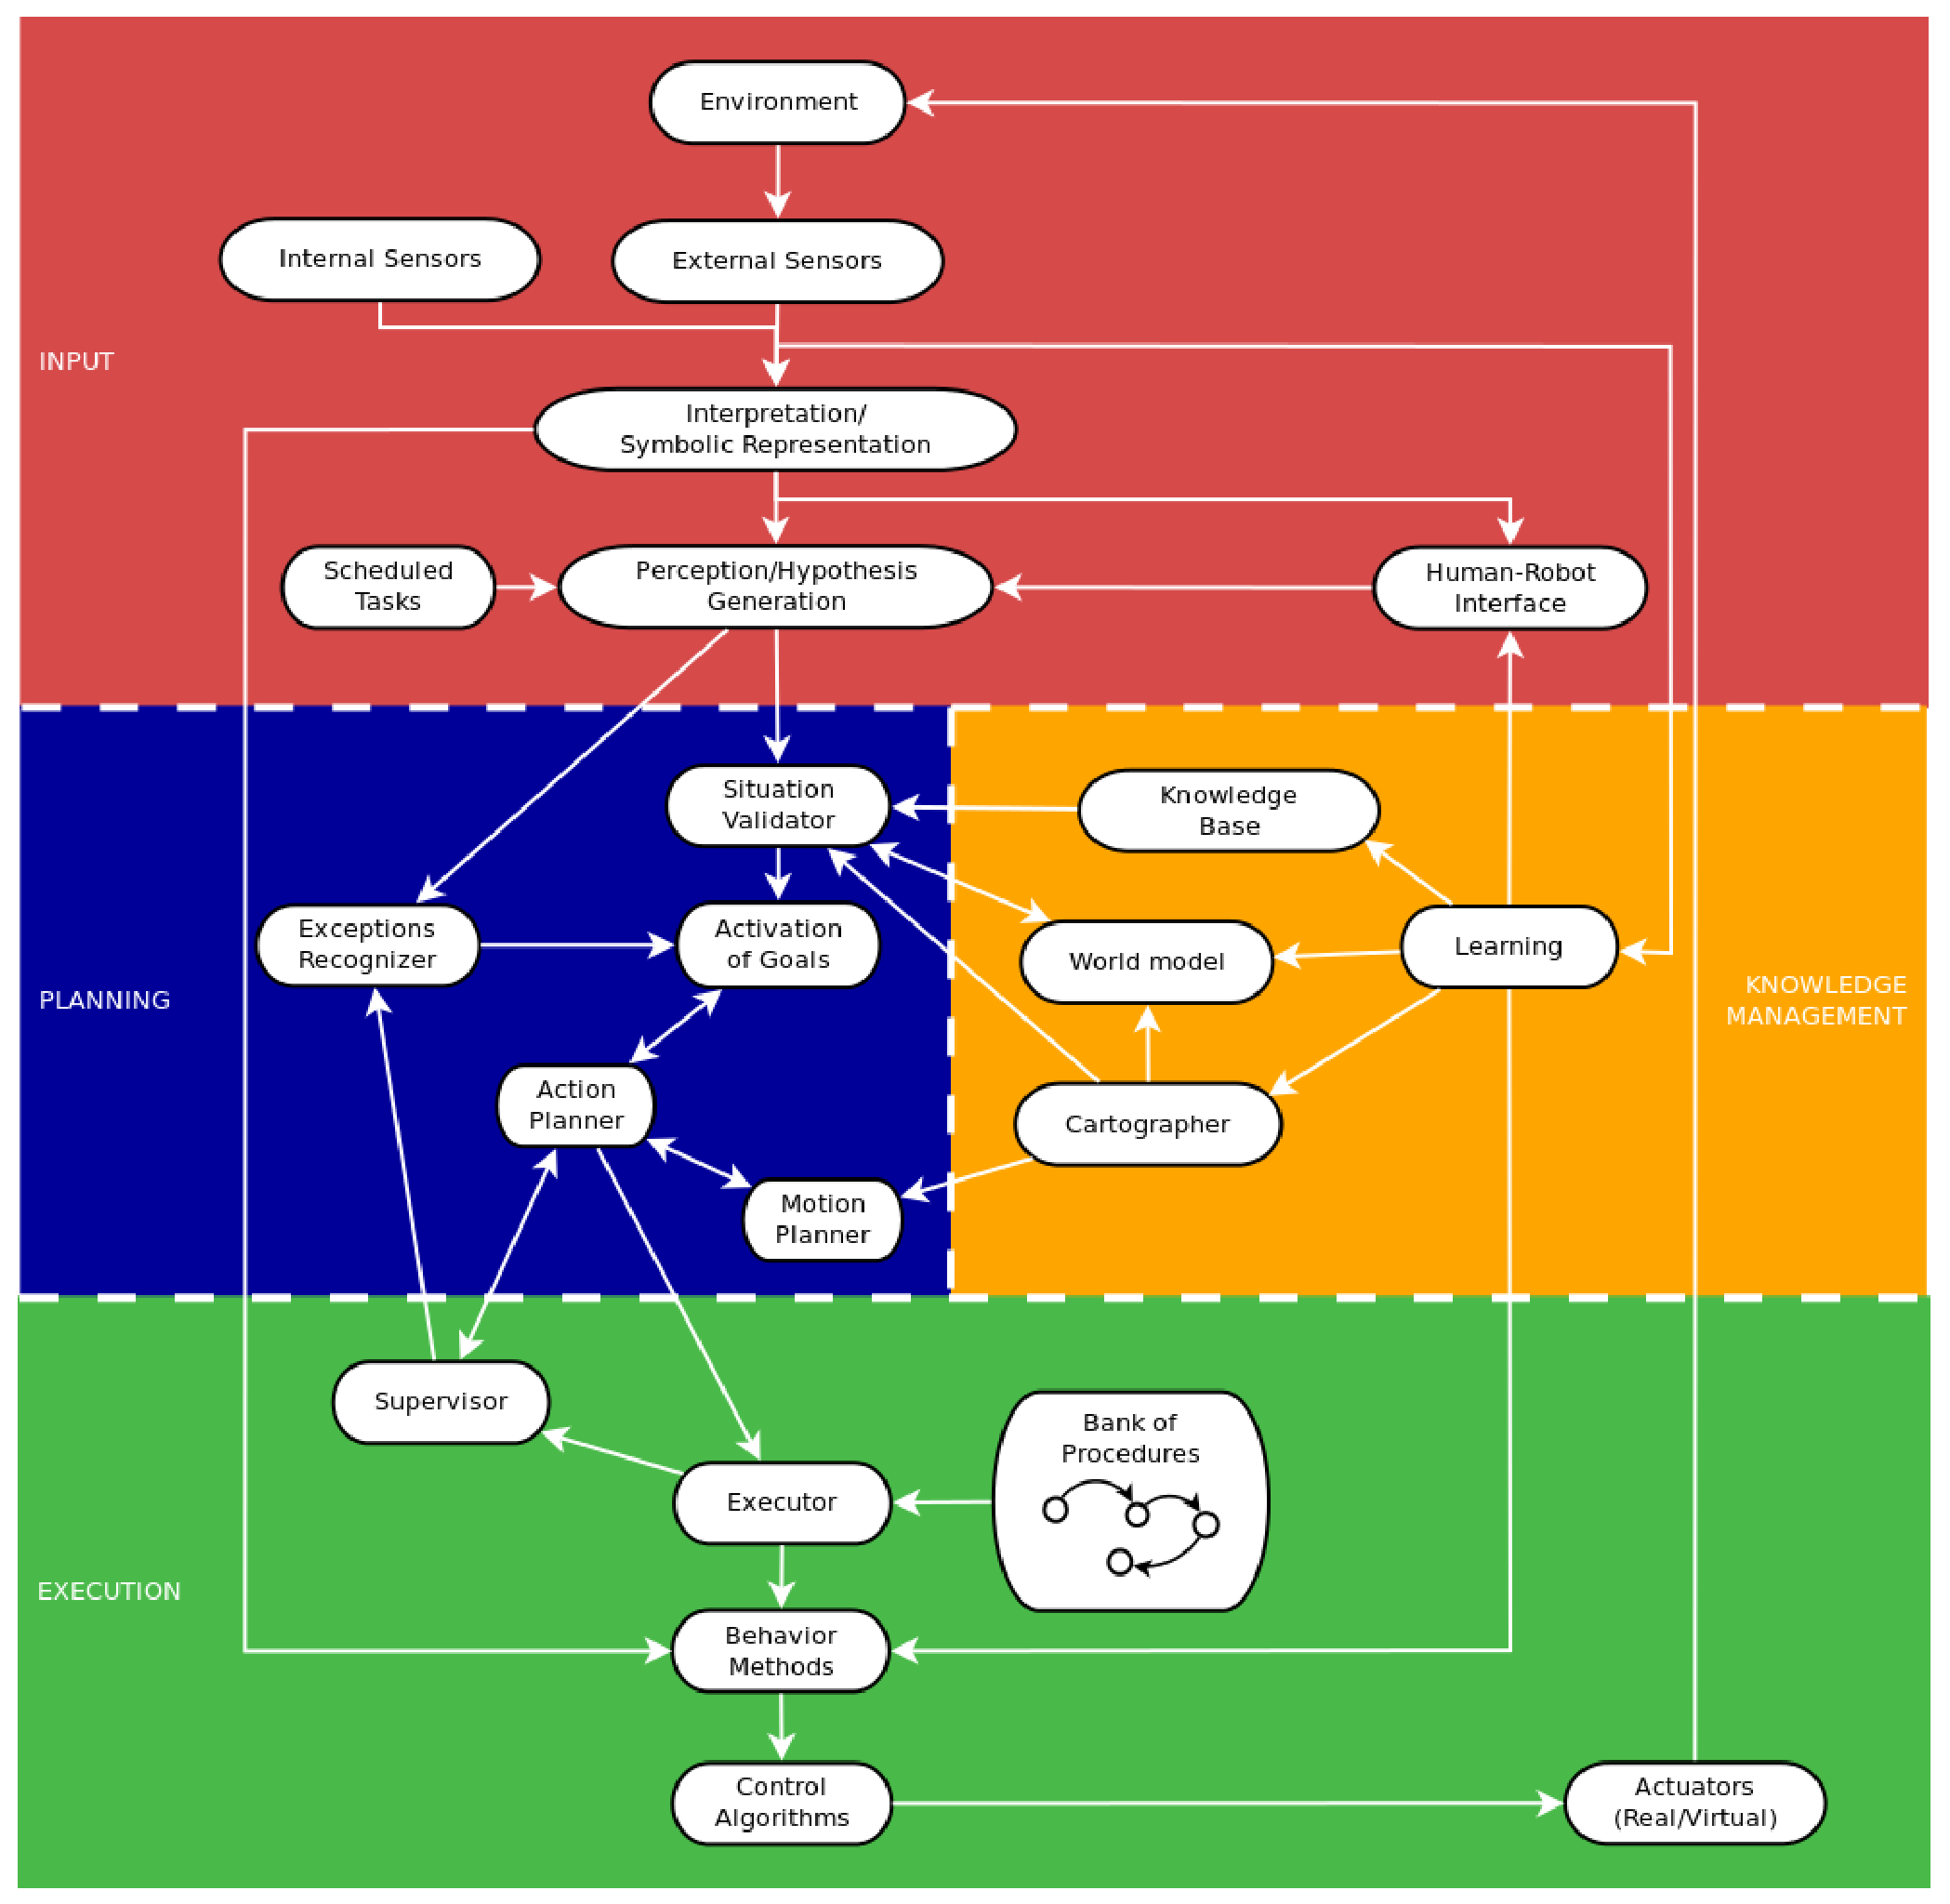
\includegraphics[angle=0, height=10cm, width=10cm]{Figures/ViRBot.eps}
	\caption{Block diagram of the ViRBot architecture.}
	\label{fig:virbot}
\end{figure}


\subsection{Inputs Layer}

This layer process the data from the robot's internal and external sensors, they provide information of the internal state of the robot, along with the external world where the robot interacts.
In some of Justina's designs it has lasers, sonars, infrared, microphones and stereo and RGB-D cameras.
Digital signal processing techniques are applied to the data provided by the internal and external sensors to obtain a symbolic representation of the data, furthermore, to recognize and to process voice and visual data.
Pattern recognition techniques are used to create models of the objects and the people that interact with the robot.
With the symbolic representation this module generates a series of beliefs, that represent the state of the environment where the robot interacts.


\subsection{Planning Layer}

The beliefs generated by the perception module are validated by this layer, it uses the Knowledge Management layer to validate them, thus a situation recognition is created.
Given a situation recognized, a set of goals are activated in order to solve it.
Action planning finds a sequence of physical operations to achieve the activated goals.


\subsection{Knowledge Management Layer}

This layer has different types of maps for the representation of the environment, they are created using 
SLAM techniques.
Also in this layer there is a localization system, that uses the Kalman filter, to estimate the robot's position and orientation.
A rule based system, CLIPS, developed by NASA, is used to represent the robot's knowledge, in which each rule contains the encoded knowledge of an expert.


\subsection{Execution Layer}
This layer executes the actions and movements plans and it checks that they are executed accordingly.
A set of hardwired procedures, represented by state machines, are used to partially solve specific problems, person recognition, object manipulation, etc. The action planner uses these bank of procedures and it joins some of them to generate a plan.


%%%%%%%%%%%%%%%%%%%
%%% CURRENT RESEARCH  %%%
%%%%%%%%%%%%%%%%%%%

\section{Current research}\label{sec:CurrentResearch}
In this section is presented the current research developed in our laboratory to improve the performance of our service robots.

\subsection{Natural language understanding}\label{subsec:NaturalLU}
Natural language understanding is used in order to the service robot interprets the language and then perform an especific task.
One of the main problems using natural language understanding is the representation of meaning.  
We have a framework for defining the semantics. The robot's semantics are therefore instructions that allow it to carry out relevant operations.

Conceptual Dependency (CD) is a theory, developed by Schank \cite{Schank}, for representing the meaning contained in sentences. 
This technique finds the structure and the meaning of a sentence in just one step. 
It is useful to represent sentences using this technique when there is not a strict grammar associated with the sentences, and also when the objective is to make inferences from them.
The CD representation of a sentence is built using conceptual primitives, these represent thoughts and the relationships between thoughts. Using conceptual dependency facilitates the use of inference rules, because many inferences are already contained in the representation itself.
There are several primitives to represent actions, for example two of the more commonly used are the following:

\vspace{.01 in}
		ATRANS: Transfer of an abstract relationship (e.g., give.)

\vspace{.01 in}
		PTRANS: Transfer of the physical location of an object (e.g., go.)
\vspace{.01 in}

Each primitive represents several verbs which have similar meaning. For instance give, buy, steal, and take have the same meaning, i.e., the transference of one object from one entity to another one.
Each primitive is represented by a set of rules and data structures. Basically each primitive contains the following components:
\vspace{.01 in}

	An Actor: He is the one that perform the ACT.
\vspace{.01 in}

	An ACT: Performed by the actor, done to an object.
\vspace{.01 in}

	An Object: The action is performed on it.
\vspace{.01 in}

	A Direction: The location that an ACT is directed towards.
\vspace{.01 in}

	A State: The state that an object is in, and is represented using a knowledge base representation as
facts in an expert system. 
\vspace{.01 in}

	For instance the phrase: {\bf "Robot, please give this book to Mary"}, 
when the verb give is found in the sentence an ATRANS structure is issued.
\vspace{.01 in}

	(ATRANS (ACTOR NIL) (OBJECT NIL) (FROM NIL) (TO NIL))
\vspace{.01 in}

The empty slots (NIL) need to be filled finding the missing elements in the sentence. The actor is the robot, the 
object is the book, etc, and it is represented by the following CD:
\vspace{.01 in}

	(ATRANS (ACTOR Robot) (OBJECT book) (FROM book's owner) (TO Mary))
\vspace{.01 in}


CDs can be use for representing simple actions. It is also well suited for representing commands or simple questions, but it is not very useful for representing complex sentences.
The CD technique were implemented in an expert system.


Much of the human problem solving or cognition can be expressed by IF THEN type production rules. Each rule corresponds to a modular collection of knowledge call chunk. The chunks are organized in loose arrangement with links to related chunk of knowledge, reasoning could be done using rules. 
Each rule is formed by a left side that needs to be satisfied (Facts) and by a right side that produce the appropriate response (Actions).  
\vspace{.01 in}

		IF  Facts  THEN  Actions.
\vspace{.01 in}

When an action is issued by a rule it may become a fact for other rules, creating links to other rules. A system may use thousands of rules to solve a problem, thus it is necessary a special mechanism that will select which rules will be fired according to the presented facts. That mechanism is an Expert System "Engine".
The Inference Engine makes inferences by deciding which rules are satisfied by facts, prioritize the 
satisfied rules, and executes the rule with the highest priority.
This expert system provides a cohesive tool for handling a wide variety of knowledge with support for three different programming paradigms: rule-based, object-oriented, and procedural.
%In the VIRBOT system an expert system maintains a knowledge data base that represents the state of the world.
The data of the humans interacting with the robot, of the objects and the locations is represented using facts that contain several slots with information related with them.
The Robot is able to perform operations like grasping an object, moving itself from on place to another, finding humans, etc. Then the objective of action planning is to find a sequence of physical operations to achieve the desired goal.
These operations are represented by a state-space graph.

In the previous example, when the user says {\bf "Robot, please give this book to Mary"}: 
\begin{itemize}
\item []
	(ATRANS (ACTOR Robot) (OBJECT book) (FROM book's owner) (TO Mary))
\end{itemize}

All the information required for the actions planner to perform its operation is contained in the CD and knowledge data base. 
Our system has been described in  \cite{iros2017} and successfully tested in robotics competitions \cite{Savage}, as the RoboCup and RockIn 
\cite{Robocup_2017}, in the category @Home.
In RoboCup@Home 2017 our robot was awarded as the best in Speech and Natural Language Understanding.



\subsection{Intelligent flat-and-textureless object manipulation in Service Robots}\label{subsec:ObjectManip}
Grasping objects from a table is a common task for Service Robots. Robots mounted with sensors suach as RGB-D cameras are able to detect the dominant plane, cluster point clouds on the plane and analyze them in order to detect the objects on it and determine the best strategy to manipulate the objects as in \cite{graspingNovelObjects} and \cite{objectDetection}. However, when the objects lack texture and or volume (i.e. flat objects), the manipulation
task becomes more challenging.


In the 2018 edition of Robocup@Home, one of the tests was the Procter \& Gamble (TM) Dishwasher Challenge (PGDC)in which they have to remove all objects from a table and place them into a dishwasher \cite{rulebook2018}. The set of objects
that were used during the test are made of plastic, without any visual pattern on them but colours with high contrast, as shown in Figure \ref{fig:rgbview}. Besides, the objects’ surface is very reflective provoking a significant variation in colour. In consequence, the information sensed by the RGB-D camera results noisy and the objects seem to belong to the table, as
shown in Figure \ref{fig:depthview}.

\begin{figure}[ht]
	\centering
	\begin{subfigure}{.225\textwidth}
  		\centering
  		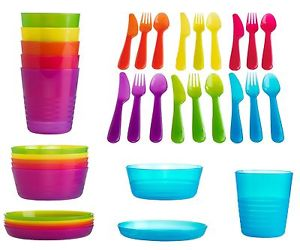
\includegraphics[width=1\textwidth]{{Figures/training_set.jpg}}
        \caption{}
  		\label{fig:rgbview}
	\end{subfigure}
	\begin{subfigure}{.225\textwidth}
  		\centering
  		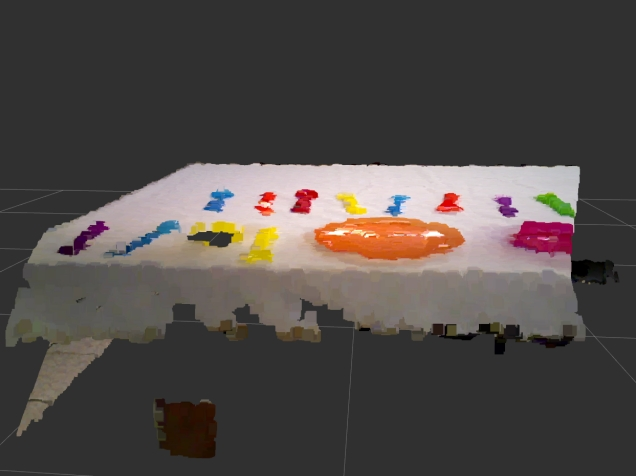
\includegraphics[width=1\textwidth]{{Figures/training0.jpg}}
        \caption{}
  		\label{fig:depthview}
	\end{subfigure}
	\caption{a) Tableware and cutlery objects used in the RoboCup@Home's P\&G Challenge and b) table setup 3D view from an RGBD camera. It can be observed that the reconstructed scene presents some errors due to sensor noise, varying illumination conditions and high object reflectance.}
	\label{fig:rgbdview}
\end{figure}

We present our solution to the flat and textureless object detection and recognition problem. We first use colour features in the detection process and then extract the geometry properties using the point cloud to describe them. This information also results useful in the manipulation process.

For background subtraction, we find the range of values in each channel on the HSV colour space for all objects and a raw segmentation mask is obtained where morphological operations of closing and dilation are applied to close the gaps where segmentation was wrong. To deal with cases where objects present significant illumination changes, a convex hull operation is applied as the final step in the segmentation process. Finally, we obtain an RGB mask and a 2D bounding box per object.

We then categorise objects into four different classes, namely glass, dish, bowl, and cutlery, by normalising the image with respect to the average depth and then extracting the area in the RGB image and the number of points and the eigenvectors from the point cloud.  An example of the classification result is shown in Figure \ref{fig:Classification}.
\begin{figure}[ht]
	\centering
	\begin{subfigure}{.425\textwidth}
  		\centering
  		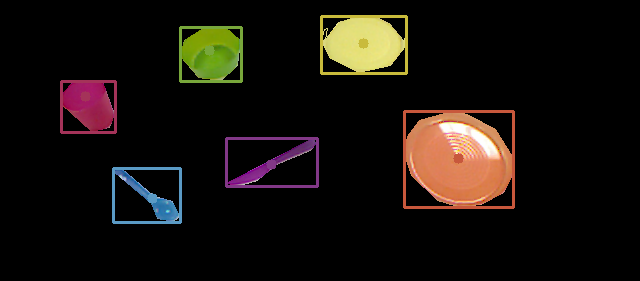
\includegraphics[width=1\textwidth]{{Figures/Segmentation.png}}
        \caption{}
  		\label{fig:seg}
	\end{subfigure}
	\begin{subfigure}{.425\textwidth}
  		\centering
  		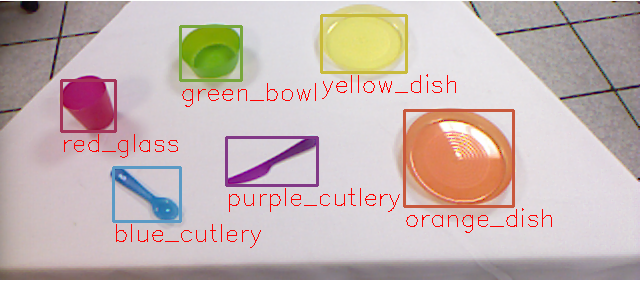
\includegraphics[width=1\textwidth]{{Figures/Classification.png}}
        \caption{}
  		\label{fig:class}
	\end{subfigure}
	\caption{a) Typical output after object detection using colour
features b) Classification result using 3D information to a setup given.}
	\label{fig:Classification}
\end{figure}


In our implementation, after the objects on the table are detected and recognised, this information is sent through ROS messages to the action planner module. The message contains information about each object, such as: a) related to the point cloud: eigenvalues, eigenvector, size, nearest point and centre point in robot coordinates, b) related to the image: position of top left corner, width and height of the bounding box, c) related to the object: centroid, roll, pitch and yaw manipulation angles, and a priority constant (this variable is set given the grasping ability of a given object with the robot hand -- the priority, in increasing order, is as follows: dish, cutlery, bowl and glass).  

Due to the size and shape of the objects in this test, we use a feedback strategy based on the visual information to verify whether the object was taken.

In the PGDC test, robot "Justina" obtained a good performance in the manipulation tasks, as we can describe in \cite{iros2018} where the robot was able to grasp 3 out of 4 objects that the robot attempted to manipulate, two of them in the first attempt, and the other in the second attempt after visual feedback confirmation was received.


 




%%%%%%%%%%%%%%%%%%%%%%%%%%
%%%  CONCLUSION AND FUTURE WORK  %%%
%%%%%%%%%%%%%%%%%%%%%%%%%%

\section{Conclusions and future work}\label{sec:conclusions}
It is clear, that during the 10 years in which our team Pumas has been participated in the RoboCup and 2 years in the Rockin \cite{Robocup_2017} in the category @Home, the performance and research developed, in the service robot area, in our laboratory has been improved considerably.
Our service robot architecture, the VIRBOT, has been evolving according to the requirement that these robotics competitions asked each year.
In these years, the full system has been improved, both in hardware and software, having reliable performance and showing promising results. Particularly, this year, we add an Embedded Develotment kit \cite{jetson} to perform GPU's solutions.
In terms of software, we have change the way of conceiving the tests of the competition: from static state machines to inferred action planning generated by a rule based system. 
As for future work, we are working in a new configuration for the omnidirectional base to improve the navigation performance. Also, we will explore new topics as the memory and enviromental reasoning of the robot, in order to explain things that hapenned in the past.
\bibliographystyle{unsrt}
\bibliography{bibliography,justina}

\begin{thebibliography}{1}


\bibitem{virbot}
{\em ViRbot: A System for the Operation of Mobile Robots}, Savage, Jesus and et al, RoboCup 2007: Robot Soccer World Cup XI,
pp 512-519, Springer Berlin Heidelberg, 2007.

\bibitem{muller}
{\em The Design of Intelligent Agents: A Layered Approach}, Muller, Jorg P,Springer-Verlag New York, Inc.1997.

\bibitem{Schank}
{\em Conceptual dependency and its descendants}, Steven L. Lytinen, Computers \& Mathematics with Applications, 1992.

\bibitem{iros2017}\textit{The Use of Expert Systems for Semantic Reasoning in Service Robots}, Jesus Savage, Julio Cruz, Reynaldo Martell, Hugo Leon, Marco Negrete, and Jesus Cruz, 2nd Workshop on Semantic Policy and Action Representations for Autonomous Robots (SPAR), IROS 2017

\bibitem{Savage}
{\em The Role of Robotics Competitions for the Development of Service Robots}, 
 Jesus Savage, Marco Negrete, Mauricio Matamoros, Jesus Cruz,
IJCAI'16, Workshop on Autonomous Mobile Service Robots, New York, USA, 2016.

\bibitem{Robocup_2017}
{\em RoboCup@Home} http://www.robocupathome.org
\\
{\em Rockin} http://rockinrobotchallenge.eu/home.php

\bibitem{graspingNovelObjects}\textit{Grasping novel objects with depth segmentation}, D. Rao, Q. V. Le, T. Phoka, M. Quigley, A. Sudsang, and A. Y. Ng, 2010 IEEE/RSJInternational Conference on Intelligent Robots and Systems, pp. 2578–2585, Oct 2010.

\bibitem{objectDetection}\textit{Object detection
based on plane segmentation and features matching for a service
robot}, A. J. R. Neves, R. Garcia, P. Dias, and A. Trifan, International Journal of Computer, Electrical, Automation, Control and Information Engineering, vol. 10, no. 4, pp. 775 – 782, 2016.

\bibitem{rulebook2018}\textit{Robocup@home 2018: Rules and regulations}, M. Matamoros, C. Rascon, J. Hart, D. Holz, and L. van Beek, 2018

\bibitem{iros2018}\textit{Intelligent flat-and-textureless object manipulation in Service Robots}, A. Ortega, H. Estrada, E. Vázquez, R. Martell, J. Hernández, J. Cruz, E. Silva, J. Savage, and L. Contreras, IROS 2018 Workshop "Towards Robots that Exhibit Manipulation Intelligence", 2018.

\bibitem{jetson}
{\em Jetson} https://developer.nvidia.com/embedded/buy/jetson-tx2-devkit

\end{thebibliography}

\section{Team Information}\label{sec:TeamInfo}
{\bf Name of Team:} 


Pumas\\
{\bf Contact Information:}


Jesus Savage


Bio-Robotics Laboratory


School of Engineering 


National Autonomous University of Mexico


robotssavage@gmail.com\\
{\bf Web Site:}


http://biorobotics.fi-p.unam.mx\\
{\bf Team Members:}


Jesus Savage, Reynaldo Martell, Hugo Estrada, Julio Cruz, Marco Negrete,


Jaime Marquez, Manuel Pano, Julio Martinez\\
{\bf Description of Hardware:}

Justina's Robotics Architecture (cf. section 2)\\
{\bf Description of Software:}

Most of our software and configurations are open-source and can found at: 

https://github.com/RobotJustina/JUSTINA\\

\begin{tabular}{l@{\extracolsep{3 cm}}  r}
 \hline                 
   Operating System & Ubuntu 16.04 LTS; Windows 7 VM \\
   Middleware & ROS Kinetic; Blackboard\\
   SLAM & ROS Gmapping\\
   Navigation & Navigation using Kinect + Ocupancy grid + A*\\
   Object Recognition & Histogram Disparity + YOLO\\
   Face Detection & Haar Cascades\\
   People Detection & OpenPoses + YOLO\\
   Face Recognition & Facenet + YOLO\\
   Speech Synthesis & Loquendo\\
   Speech Recognition & Microsoft Speech Recognition\\
   Inference Engine & CLIPS\\
 \hline  
 \end{tabular}
	


\end{document} 
